\chapter{Preparation}

\section{Theory}

\subsection{Slab Waveguide}
\subsubsection{Calculation of Modes}
\subsubsection{Field Distribution and Dispersion Diagramm}


\subsection{Strip Waveguide}



\section{Questions}

\subsection{Slab and Strip waveguide?}
\label{q1}
A slab waveguide is a structure of several layers of different materials. The structures are extended infinitely. The middle layer has the highest refractive index. Here the electric field is confined and the wave is guided.
Figure \ref{fig:slab} shows the schematic layout of a slab waveguide and the index profile of this structure. 
As materials and therefore refractive indices for the cladding and the Substrate SiO$_2$ with $n_2 = 1.44$ is selected. For the core region the refractive index of Silicon with $n_1 = 3.48$ is selected.

\begin{figure}%
\centering
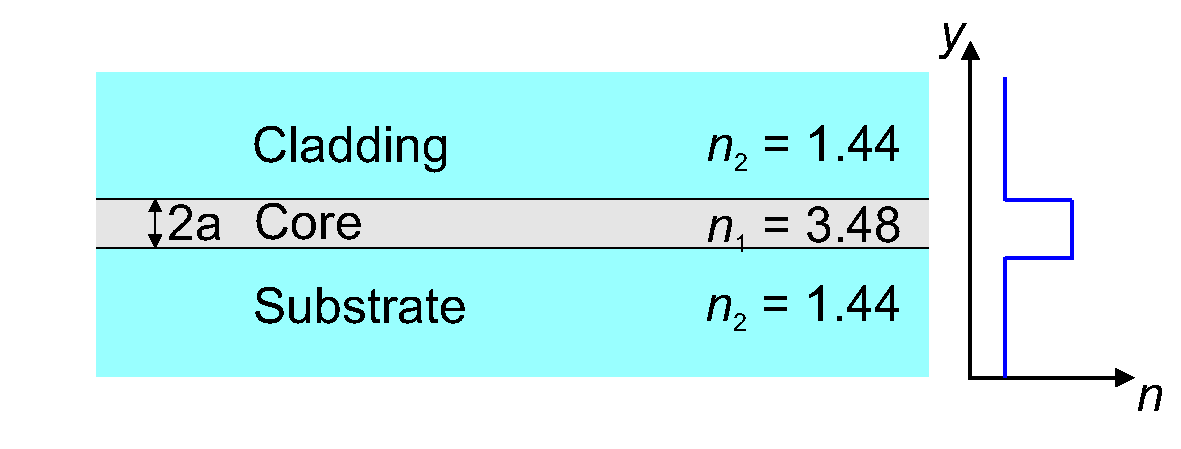
\includegraphics[width=.7\columnwidth]{Grafiken/swg.pdf}%
\caption{schematic layout of a slab waveguide}%
\label{fig:slab}%
\end{figure}

In contrast there is the strip waveguide. Here a strip of high-index material is placed on a lower index substrate. On top sometimes is a polymer or just air. Figure \ref{fig:strip} shows the schematic layout of a strip waveguide and the index profile at the marked position $x = 0$.

\begin{figure}%
\centering
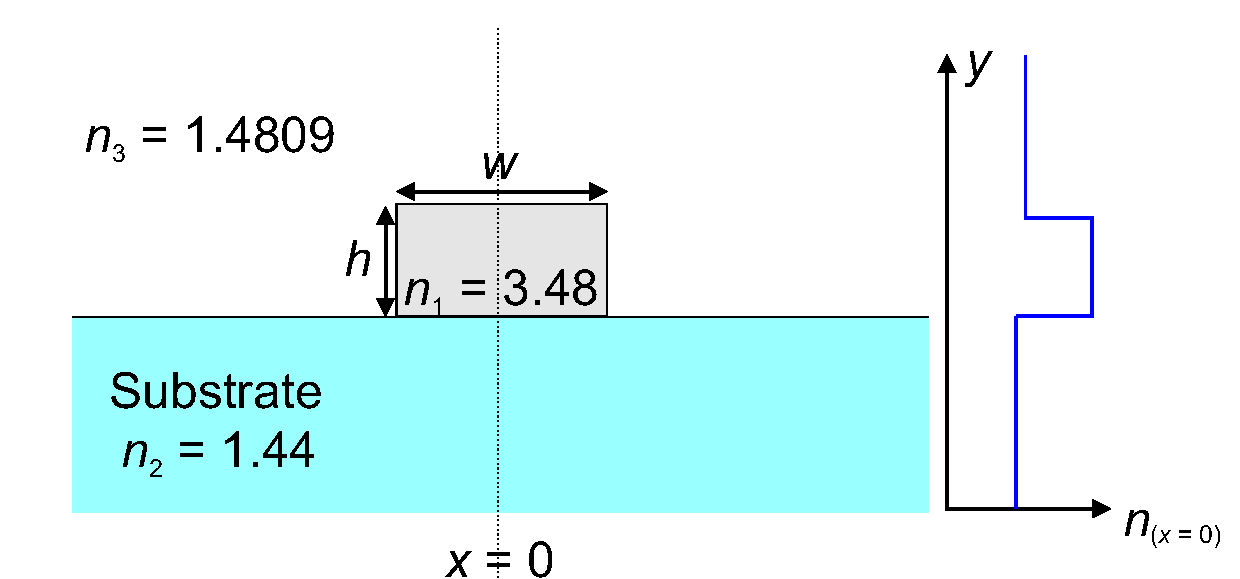
\includegraphics[width=.7\columnwidth]{Grafiken/strip.pdf}%
\caption{schematic layout of a strip waveguide}%
\label{fig:strip}%
\end{figure}

\subsection{Different performance between TE and TM @ boundary}
There are different kinds of polarizations. The TE-polarized wave has the boundary conditions:\\
$\vec{\mathrm{E}}_i ~\bot~$plane of incidence\\
and\\
$\vec{\mathrm{H}}_i ~||~$ plane of incidence.\\

For the TM-polarized wave the following boundary conditions are given:\\
$\vec{\mathrm{H}}_i ~\bot~$plane of incidence\\
and\\
$\vec{\mathrm{E}}_i ~||~$ plane of incidence.\\
Any other polarization states can be interpreted as a superposition of a TE and a TM wave.

The TE-modes have always a larger propagation constant than the TM-modes. TE-modes are more confined to the high-index core region than the TM modes.\footnote[1]{Christian Koos, Optical Waveguides and Fibres, Lecture Notes}


\subsection{Single Mode strip waveguide}

\begin{figure}%
\centering
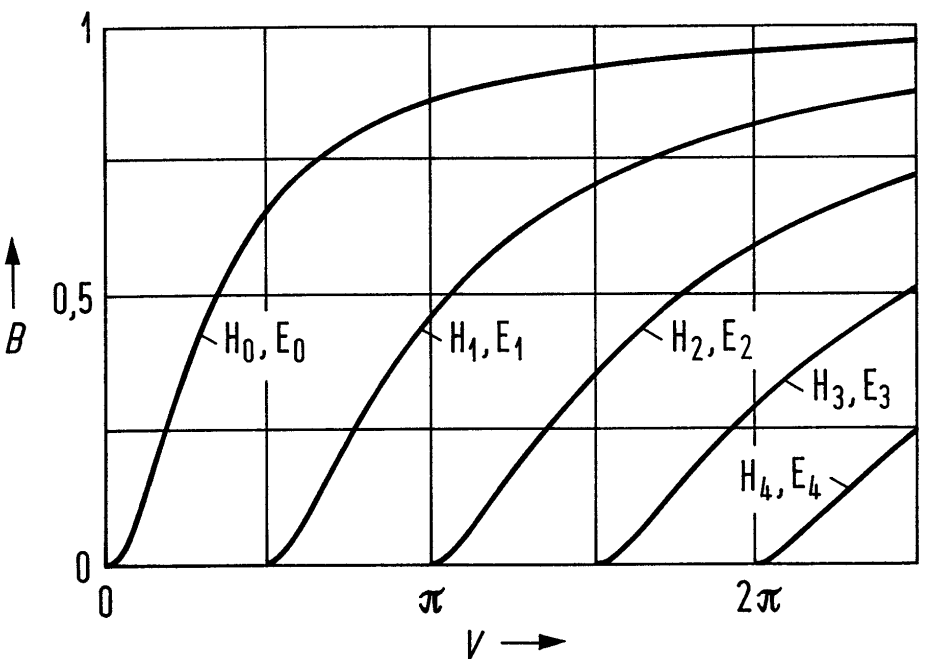
\includegraphics[width=.5\columnwidth]{Grafiken/SingleMode.png}%
\caption{Normalized propagation $B$ over normalized frequency $V$ for a low index contrast.}%
\label{fig:singlemoded}%
\end{figure}
To achieve a single mode strip waveguide the normalized frequency $V$ needs to be smaller than $V=\pi/2$. As in Figure \ref{fig:singlemoded}\footnote[2]{Wolfgang Freude, Optische Wellenleiter und Sender, Lecture Notes} shown for $V < \pi/2$ only the fundamental mode can propagate. There are still two polarizations H$_0$ and E$_0$.

Using \begin{equation}
V=ak_0\sqrt{n_1^2-n_2^2}
\label{eq:norm_freq}
\end{equation}
with $2a$ is the thickness of the core, $n_1$ is the refractive index of the core, $n_2$ is the refractive index of the surrounding material and $k_0$ is the wavenumber, the the requirements to the waveguide design can be derived.
For the in \ref{q1} assumed values for $n_1$ and $n_2$ this leads to a core-thickness of
\begin{equation}
2a>\frac{\pi}{k_0\sqrt{n_1^2-n_2^2}}=\frac{\lambda_0}{2\sqrt{n_1^2-n_2^2}}=2.45~\cdot~10^{-7}~\mathrm{m}
\label{eq:}
\end{equation}
for $\lambda_0$ = 1550~nm, $n_1 = 3.48$ and $n_2 = 1.44$. 
That means when using a Silicon core with a hight of 245~nm the slab waveguide is single moded f�r $\lambda_0 < 1.55~\upmu$m.
